\documentclass[draft]{aiaa-pretty}
\usepackage{graphicx}
\usepackage{pdfpages}
\usepackage{float}
\usepackage{epstopdf}
% Author information
\author{ % and
Jonathan Thorne\thanks{Masters Student, AIAA Student Member}, 
Aaron Katz\thanks{Assistant Professor, AIAA Member}, 
Oisin Tong\thanks{PHD Candidate, AIAA Student Member},
and Yushi Yanagita\thanks{Masters Student, AIAA Student Member}\\
\textit{Department of Mechanical and Aerospace Engineering, Utah State University, Logan, UT 84322}}
% Title
\title{High-Order Strand Grid Methods for Low Mach and Incompressible Flows}
%Abstract


\abstract{ %
A novel high-order finite volume scheme using flux correction methods in conjunction with structured finite difference schemes is 
extended to low Mach and incompressible flows on strand grids.  Flux correction achieves high order by using correction terms in the 
fluxes in and out of each finite volume cell.  The flux correction method is applied in unstructured layers of the 
strand grid, the layers are then coupled together using a source term containing the derivatives in the strand direction.  Strand-
direction derivatives are obtained by using summation-by-parts operators for the first derivative and variable coefficients for the
second derivatives.  A preconditioner is used to increase the applicability of the method to low Mach and incompressible flows.  Verification
is completed using the method of manufactured solutions.  The method is extended with the introduction of a Spalart Allmaras turbulence model.
Results found for low-Mach and incompressible flows and is compared to analytical and experimental data.
        }
\begin{document}
\maketitle

\section{Introduction}
Low Mach number flows present many difficulties to compressible computational fluid dynamics (CFD) algorithms in terms of accuracy and convergence rate.  
Many of these flows have widely varying particle and acoustic speeds, degrading solution convergence \cite{Folkner2014}.  Artificial dissipation
using second-order CFD methods often reduces the accuracy of the solution, so even when convergence is achieved the solution could be
inaccurate.  As an added challenge, complex geometry presents difficulties for mesh generation.  Meshing can take days or weeks
depending on the complexity of the geometry.  Progress addressing these challenges can lead to transformational changes for many applications, such as underwater vehicle design.

First, to improve accuracy and convergence for low Mach and incompressible flows preconditioning is often needed.  Preconditioning has also shown to be beneficial in flows that 
have low speed flow regions, such as in boundary layers or at stagnation points. In addition, preconditioning enables the use of arbitrary state equations providing 
solutions for real gas effects, multiphase flows, and combustion \cite{Merkle1998}.

Second, to reduce numerical diffusion a high-order method is needed.  Flux correction (FC) was recently introduced by Katz and Sankaran \cite{Katz2012} that provides high-order 
spacial accuracy in conjunction with the need for only first-order derivative terms \cite{Katz2013,Delanaye1999}.  High-order accuracy is achieved by correction terms in the flux 
between nodes, creating a method that has low computational overhead with high-order results.  This method has been shown to be third-order on arbitrary triangular meshes for 
inviscid flows \cite{Katz2012} and approaches fourth-order in highly viscous flows \cite{Katz2013}.

Third, to address complex geometry, strand meshing has shown great potential.  Using a strand mesh has been shown to alleviate many difficulties by being
able to fully automate volume grid generation.  The strands are automatically generated by using a pointing vector developed from a surface tessellation.  The strands are 
then split into segments creating layers of unstructured mesh layers.  Over these layers the high-order method is applied.  Strand meshing simplifies the
meshing process and increases automation, as well as providing a high-order mesh for the use of high-order methods.  In addition, with strand meshing techniques 
self-satisfying domain connectivity (SSDC) is possible, where each processor in a multi-processor computation has access to the entire domain while only needing 
minimal information.

By using the methods described solutions for low-Mach and incompressible flows will be explored.  This work is outlined such that the first section contains the numerical
methods needed to create the preconditioner, the addition of the turbulence model, the discretization and transformations needed for a strand meshing method, and a brief description
of Flux Correction. 
The next section provides results
using the methods described in the numerical methods portion.  Finally, conclusions are found and work for the future work is addressed.

\section{Numerical Methods}
\subsection{Traditional Preconditioning}
Numerous matrix preconditioning methods based on matrix dissipation have already been utilized successfully by other researchers to improve performance of compressible CFD
methods in low Mach and incompressible regimes \cite{Folkner2014,Weiss1995,Caughey2003}.  We will present traditional framework for most preconditioning schemes in
three-dimensions.  Following the notation of Merkle, et al. \cite{Merkle1998}, the Naiver-Stokes equations without source terms are expressed
as
% Look Thru this and change to Navier-Stokes equations rather the Euler %
\begin{equation}
\frac{\partial Q}{\partial \tau} + \frac{\partial F_j}{\partial x_j} - \frac{\partial F_j^\nu}{\partial x_j} = 0,
\label{Euler}
\end{equation}
where Q represents the matrix of conserved variables, $\tau$ represents the pseudo-time, and $F_j = (F, G, H),$ is the inviscid fluxes, and $F^\nu_j = (F^\nu,G^\nu,H^\nu)$ represents the viscous fluxes.

\begin{equation}
  Q = \begin{Bmatrix}
    \rho \\ \rho u_i \\ \rho E
  \end{Bmatrix}, \quad
  F_j = \begin{Bmatrix}
    \rho u \\ \rho u_iu_j + p\delta_{ij} \\ \rho h u_j
  \end{Bmatrix}, \quad
  F^\nu_j = \begin{Bmatrix}
    0 \\ \sigma_{ij}  \\ \sigma_{ij}u_i-q_j
  \end{Bmatrix}.
\end{equation}
The variables include $\rho$, $u_j = (u,v,w)$, $E$, $p$ and $h^0$, which represent density, velocity in the $j^{th}$ direction, total energy per unit mass,
and enthalpy per unit mass, respectively. $\delta_{ij}$ is the chronicler delta and $\sigma_{ij}$ is the deviatoric stress tensor. $q_j$ is the $j^{th}$ component of the 
heat flux vector.
The stress tensor is defined as

\begin{equation}
\sigma_{ij} = 2\mu\left(S_{ij}-\frac{1}{3}\frac{\partial u_k}{\partial x_k}\delta_{ij}\right), 
\end{equation}
where $\mu$ is the dynamic viscosity and $S_{ij}$ is the rate of strain tensor, defined as
\begin{equation}
 S_{ij}=\frac{1}{2}\left(\frac{\partial u_i}{\partial x_j}+\frac{\partial u_j}{\partial x_i}\right).
\end{equation}


Preconditioning methods often begin with a conversion from the conserved variables to primitive variables,
\begin{equation}
 Q_v = \begin{Bmatrix}
        \rho \\ u_j \\ T
       \end{Bmatrix},
\end{equation}
where $Q_v$ is the matrix of primitive variables and $T$ is temperature.  This is done to simplify the preconditioning process.  Conversion between the primitive variables
and the conserved variables are completed via the Jacobian matrix,
\begin{equation}
 \Gamma \equiv \frac{\partial Q}{\partial Q_v} =   
 \begin{pmatrix}
    \rho_p                  & 0      & 0      & 0		& \rho_T           \\
    u\rho_p                 & \rho   & 0      & 0		& u\rho_T           \\
    v\rho_p				    & 0		& \rho	 &  0		& v\rho_T		     \\
    w\rho_p				    & 0		& 0		 &  \rho		& w\rho_T		      \\
    h^0\rho_p + \rho h_p -1 & \rho u & \rho v & \rho w   & h^0\rho_T + \rho h_T \\
  \end{pmatrix},
\end{equation}
where subscripts $p$ and $T$ denote partial differentiation (e.g. $\rho_p = \frac{\partial \rho}{\partial p}$).  The goal of the preconditioner is to reduce wave speeds 
disparities, provide well poisedness, and ensure diagonal dominance. This is done by replacing the matrix $\Gamma$ in the pseudo-time derivative term with a preconditioning 
matrix $\Gamma_p$.
\begin{equation}
  \Gamma_p =    
 \begin{pmatrix}
    \rho'_p                  & 0      & 0      & 0		& \rho_T           \\
    u\rho'_p                 & \rho   & 0      & 0		& u\rho_T           \\
    v\rho'_p				    & 0		& \rho	 &  0		& v\rho_T		     \\
    w\rho'_p				    & 0		& 0		 &  \rho		& w\rho_T		      \\
    h^0\rho'_p + \rho h_p -1 & \rho u & \rho v & \rho w   & h^0\rho_T + \rho h_T \\
  \end{pmatrix},
\label{PreconJacobian}
\end{equation}
it is observed that $\Gamma_p$ is identical to $\Gamma$ except for the new $\rho'_p$ term.  The selection of $\rho'_p$ is accomplished by forcing the acoustic wave speed to
be the same order of magnitude as the particle speeds. Sankaran \cite{Venkateswaran1999} and Merkle, et al. \cite{Merkle1998} both take this approach and note the existence of 
a preconditioned speed of sound,
\begin{equation}
 V_p^2 \equiv \frac{\rho h_t}{d'}
 \label{SpeedofSound}
\end{equation}
where $d'$ is defined as
\begin{equation}
 d' \equiv \rho h_T \rho'_p+\rho_T\left(1-\rho h_p \right).
\end{equation}
The convergence and dissipation scaling properties of the preconditioner are dependent
primarily on the preconditioned speed of sound chosen.  Traditionally this is chosen via the particle speed, 
\begin{equation}
 V_p = \sqrt{\left(u^2+v^2+w^2\right)}.
\end{equation} 

\subsection{Optimally Defined Preconditioning}
In many flows, there exists many different wave speeds.  Because $\Gamma_p$ is a local value, it is possible to make a definition of the preconditioner that is optimally defined
such that convergence is improved in the entire domain.  This optimally defined preconditioning scheme would be able to switch on and off dependent on the nessesity of the flow, based
on the particle speed.
This is done through the definition a preconditioned Mach number,
\begin{equation}
\begin{aligned}
 M_p &= \begin{cases} 
      \sqrt{\frac{2M^2}{1-2M^2}} & M<.5\\
      1 & M \geq .5 
   \end{cases},\\
 V_p &= M_pc,
\end{aligned}
\end{equation}
where $M_p$ is the preconditioned Mach number, $M$ is the local Mach number, and $c$ is the speed of sound.  With this definition the inviscid eigenvalues are defined as
\begin{equation}
\begin{aligned}
\label{eigenvalues}
 \lambda_{1,2}&=\frac{1}{2}\left(u_n\left(1+M_p^2\right)\pm\left(u_n^2\left(M_p^2-1\right)^2+4V_p^2\right)\right),\\
 \lambda_{3,4,5}&=u_n.
\end{aligned}
\end{equation}
When $M_p>.5$ then the standard compressible eigenvalues are returned, however, when the flow is incompressible the eigenvalues introduce an artificial compressibility constant.  
This is analogous to the compressibility term introduced by Chorin \ref{}.  With this optimally defined system both incompressible and compressible functionality can be achieved.  
In addition, convergence will be improved in flows that contain stagnation points, or regions of low-speed flow.

%\begin{equation}
%  V^u_p = \min\left(\max\left(\sqrt{u^2 + v^2},\mbox{Str}\sqrt{u^2 + v^2}\right),
%  c\right).
%\end{equation}
%Where $\mbox{Str}$ is the Strouhal number which represents a non-dimensional frequency of the dominate unsteady physics in the flow,
%\begin{equation}
% \mbox{Str} = \frac{L}{\pi \Delta t \sqrt{u^2+v^2}},
%\end{equation}
%and $c$ represents the speed of sound in the fluid.  By specifying a preconditioned speed of sound, Equation \ref{SpeedofSound} provides a definition of $\rho'_p$ found in the preconditioned
%conserved variables Jacobian in Equation \ref{PreconJacobian}.  $\rho'_p$ is now defined as 
%\begin{equation}
% \rho'_p = \frac{1}{V^2_p}-\frac{\rho_T \left( 1-\rho h_p\right)}{\rho h_T}.
%\end{equation}

% Talk about relationship between rho' and preconditioned speed of sound
%By choosing the correct value for the preconditioned speed of sound accurate scaling in the fluid can achieve.  This in turn provides better convergence overall and more accuracy in
%low Mach number and incompressible flows. 
\subsection{Addition of Spalart Allmaras Turbulence Model}
Oisin will probably write this...

\subsection{Flux Correction High-Order Method}
High-order flux correction is a third-order spatially accurate method developed by Katz and Sankaran \cite{}.  A more complete derivation is contained in other works \cite{}, but
for completeness, a brief derivation is included.  Flux correction involves adding a correction term to the fluxes, such as its name suggests. Looking at the inviscid fluxes and 
dissipation,

\begin{equation}
 \mathcal{F}^h_{0i}=\frac{1}{2}\left(\mathcal{F}_0+\mathcal{F}_i\right)-\frac{1}{2}\left|\Gamma^{-1}\mathcal{A}\left(Q_R,Q_L\right)\right|\left(Q_R-Q_L\right).
\end{equation}
Where $\mathcal{F}$ is the inviscid fluxes doted with the unit normal, $0$ and $i$ denote the node, $\mathcal{A}=\partial\mathcal{F}/\partial\mathcal{Q}$ is the directed flux 
Jacobian, and $Q_R$ and $Q_L$ are the conserved variables at the left and right node.  Note that the preconditioning matrix $\Gamma$ is introduced into the artificial dissipation term.
the directed flux Jacobian can be broken into the left and right eigenvectors and the eigenvectors,
\begin{equation}
 \left|\Gamma^{-1}\mathcal{A}\right| = M\left|\lambda\right|M^{-1},
\end{equation}
where the eigenvalues are  given in Equation \ref{eigenvalues}.  The right and left flux and dissipation terms are given by
\begin{equation}
 \begin{aligned}
  F_L &= \mathcal{F}_0 + \frac{1}{2} \mathbf{\Delta r}^T \mathbf{\nabla}^h, \\
  F_R &= \mathcal{F}_i  - \frac{1}{2} \mathbf{\Delta r}^T \mathbf{\nabla}^h, \\
  Q_L &= Q_0 + \frac{1}{2} \mathbf{\Delta r}^T \mathbf{\nabla}^h Q_0,\\
  Q_R &= Q_i - \frac{1}{2} \mathbf{\Delta r}^T \mathbf{\nabla}^h Q_i,\\
 \end{aligned}
\end{equation}
where $\mathbf{r}$ is the position vector along the edge.  The gradient is discretized as 
\begin{equation}
\mathbf{\nabla}^h = \mathbf{\nabla} + O(h^p)
\label{Gradient},
\end{equation}
where $p$ is the order of accuracy, and $O(h^p)$ denotes the truncation error of the gradient procedure.  For flux correction, the order of accuracy of the flux and solution gradients 
must be at least second-order to maintain consistency ($p\ge2$).  The advantage of flux correction over other high-order methods is that it bypasses the  need for second derivatives and
does not require high-order quadrature.  This makes the method an efficient way to achieve third-order accuracy without excess computational expense.

\subsection{Strand Grid Methods}
 Strand grids show great potential in modern CFD.  They provide a method for consistent mesh generation and automation.  Strands are produced by crating a surface tessellation from which
 straight lines (strands) are extruded emanating from the surface.  This creates the potential for easy scalability, as the strands are developed from the surface structure and emanated 
 out.  These strands are then broken into levels generating surfaces in the mesh.  This can be seen in Figure \ref{Strand},
 where each clipping index defines a new surface mesh. 
 \begin{figure}
  \centering
  %\includegraphics[scale=.5]{Figures/Strand.pdf}
  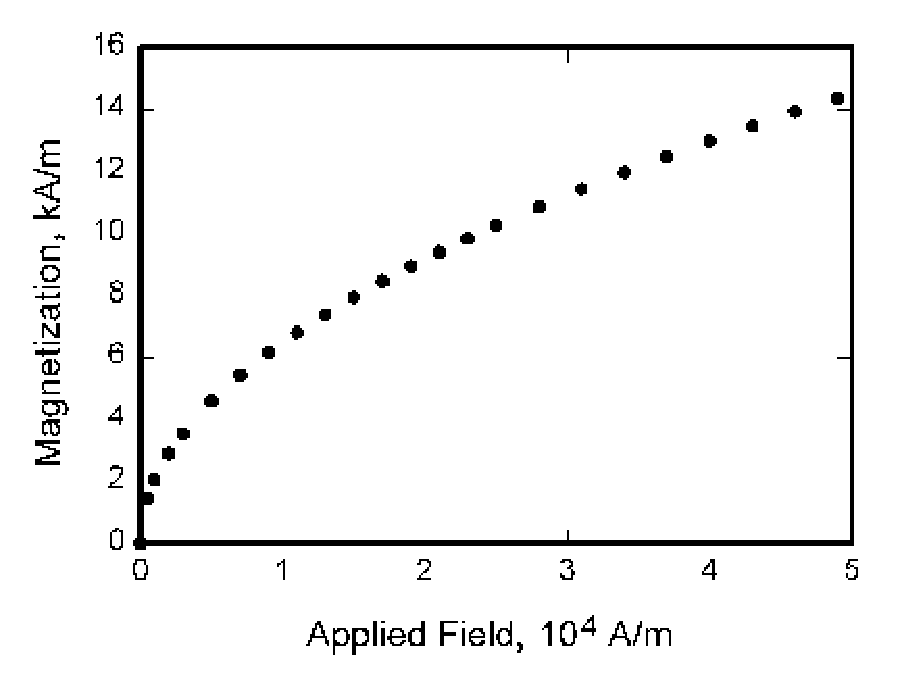
\includegraphics[scale=.5]{figure_magnet.eps}
  \caption{Example of strand mesh extrusion \label{Strand}}
 \end{figure}
 
 After initial mesh generation, each level of the mesh is then transformed into the computational domain, seen in Figure \ref{CompDom}. In the computational space $\Delta \eta = 1/(N-1)$.
 Upon transformation to computational space Equation \ref{Euler} becomes
 \begin{equation}
  \frac{\partial \hat{Q}}{\partial t}+\frac{\partial \hat{F}}{\partial r}+\frac{\partial \hat{G}}{\partial s}+\frac{\partial \hat{H}}{\partial \eta}
  -\frac{\partial \hat{F}^\nu}{\partial r}-\frac{\partial \hat{G}^\nu}{\partial s}-\frac{\partial \hat{H}^\nu}{\partial \eta}=\hat{S} \label{ComSpace}
 \end{equation}
 where $\hat{Q}$, $\hat{S}$, $\hat{F}$, $\hat{G}$, $\hat{H}$, $\hat{F}^\nu$, $\hat{G}^\nu$, and $\hat{H}^\nu$ and the transformation matrix are defined as,
 \begin{gather*}
  \hat{Q} \equiv JQ, \quad \hat{S} \equiv JS, \\
  \hat{F}\equiv J \left(r_xF+r_yG+r_zH\right), \quad \hat{F}^\nu \equiv J\left(r_xF^\nu+r_yG^\nu+r_zH^\nu\right),  \\
  \hat{G}\equiv J \left(s_xF+s_yG+s_zH\right), \quad \hat{G}^\nu \equiv J\left(s_xF^\nu+s_yG^\nu+s_zH^\nu\right),  \\
  \hat{H}\equiv J \left(\eta_xF+\eta_yG+\eta_z H\right), \quad \hat{H}^\nu \equiv J\left(\eta_xF^\nu+\eta_yG^\nu+\eta_zH^\nu\right), \\
  \left(\begin{matrix}
   r_x & s_x & \eta_x \\
   r_y & s_y & \eta_y \\
   r_z & s_z & \eta_z \\
  \end{matrix}\right) = \frac{1}{J} \left( \begin{matrix}
  y_sz_\eta - z_sy_\eta & z_ry_\eta - y_rz_\eta & y_rz_s-z_ry_s \\
  z_sx_\eta - x_sy_\eta & x_rz_\eta - z_rx_\eta & z_rx_s-x_rz_s \\
  x_sy_\eta - y_sx_\eta & y_rx_\eta - x_ry_\eta & x_ry_s-y_rx_s \\
  \end{matrix} \right), \\
  J = x_\eta\left( y_rz_s-z_ry_s\right) + y_\eta\left( z_rx_s - x_rz_s \right) + z_\eta(x_ry_s-y_rx_s).
 \end{gather*}
 \begin{figure}
  \centering
  %\includegraphics[scale=.5]{Figures/Transform.pdf}
  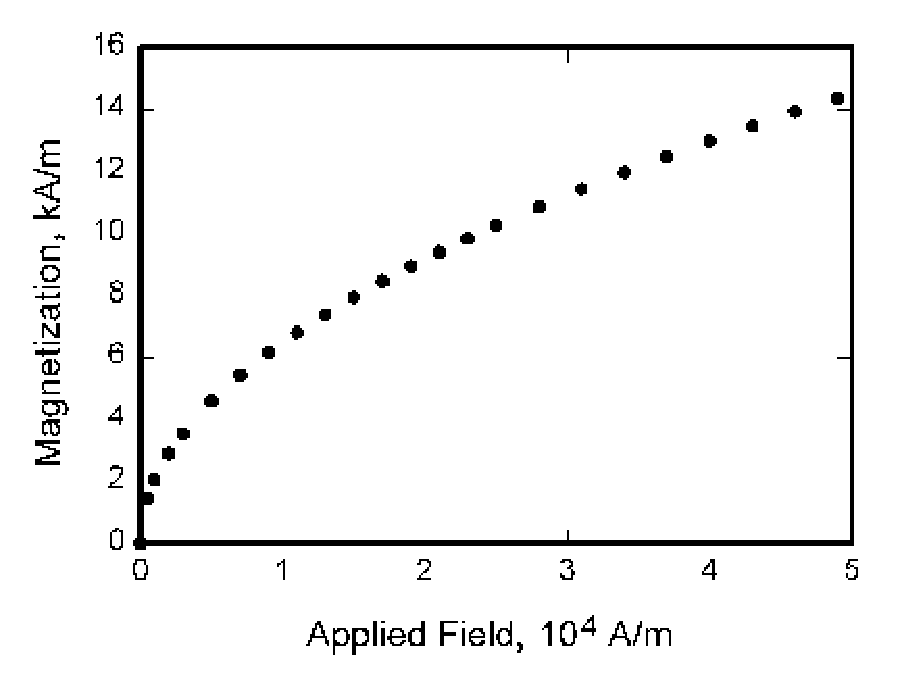
\includegraphics[scale=.5]{figure_magnet.eps}
  \caption{Transformation between physical and computational domains \label{CompDom}}
 \end{figure}
 Here, J is the Jacobian of the transformation, and partial differentiation is denoted with a subscript (e.g. $\partial x/\partial s = x_s$).  
 
 After transformation,
 each strand layer is then connected by using high-order finite differences based on summation-by-parts along the $\eta$ direction for the first derivatives then uses 
 variable coefficients for the second derivatives. Along the r-s plane high-order FC will be implemented.  The r-s plane is then combined with the $\eta$ direction by a source term.
 This source term can be found by rearranging Equation \ref{ComSpace} and moving the $\eta$-derivatives to the left side of the equation with the source terms, resulting in
 \begin{equation}
  \frac{\partial \hat{Q}}{\partial \tau}+\frac{\partial \hat{F}}{\partial r}+\frac{\partial \hat{G}}{\partial s}
  -\frac{\partial \hat{F}^\nu}{\partial r}-\frac{\partial \hat{G}^\nu}{\partial s}=\tilde{S},\label{Simple}
 \end{equation}
 \begin{gather*}
  \tilde{S} \equiv \hat{S} - \frac{\partial \hat{Q}}{\partial t} - \frac{\partial \hat{H}}{\partial \eta} + \frac{\partial \hat{H}^\nu}{\partial \eta}. 
 \end{gather*}
 
 Because of this transformation done in Equation \ref{Simple}, the problem is simplified to essentially a two dimensional problem combined with source terms.  This becomes 
 convenient when the method is later parallelized when solving the problem, as it creates a situation of SSDC.  Because of the simplicity of the mesh and the need to only 
 do computations in the two-dimensional domain each processor can have access to its own mesh. Processor interactions are minimized by only needing the source terms, 
 increasing computational speed with multiple processors.
 
% % Add SSDC and Equations for r-s-eta transformation


\section{Results}

\subsection{Analytical Verification}
\subsubsection{MMS Verification}
Me
\subsubsection{Creeping Flow}
Me

\subsection{Experimental Verification}
\subsubsection{Reynolds Sweep with Sphere}
Me
\subsubsection{Turbulent Low-Mach Flow over Body 1}
Yushi
\subsubsection{Turbulent Incompressible Flow over Model 4155}
Yushi
\subsubsection{Turbulent Incompressible Flow over Model 4159}
Yushi

% % Add results of boundary layer with the results of the plate
% Verification of the three dimensional version of FC was completed using the method of manufactured solutions (MMS).  Smooth trigonometric functions where used to develop 
% the velocity, temperature, and pressure profiles as shown in figure \ref{MMS}.  The values of each as a maximum variation around 10\%.
% Four grid levels where used to determine the order of accuracy of the method by measuring error of the solution against the exact solution after convergence to machine 
% zero is achieved.  Mesh was randomly perturbed to show the convergence on a random mesh. Results of the study are shown in figure \ref{MMSresults}. Cases showing the results 
% of inviscid and viscous terms are shown in isolation, as well as a combination of the two.  The study was conducted with $Re = 10$.  The reason for showing the viscous, 
% inviscid, and combined convergence is to further verify the fourth order convergence of FC in a viscous domain, and to show third order convergence in the inviscid domain.
% 
% \begin{figure}
% \centering
% \includegraphics[scale=.5]{MMS.pdf}
% \caption{\label{MMS} Manufactured solution used for order of accuracy verification}
% \end{figure}
% 
% \begin{figure}
% \centering
% \includegraphics[scale=.5]{MMSResults.pdf}
% \caption{\label{MMSresults} Order of accuracy results for manufactured solution in a cube geometry}
% \end{figure}
% 
% Boundary layer application was tested in two-dimensions with a flat plate in a flow with Mach = 0.2 and with a Reynolds number of $10^4$.  For this case we used a semi-coarse mesh containing
% 96 nodes along the plate surface and 32 nodes normal to the plate, with a wall spacing of 2 x $10^-4$.  The domain starts with a short inviscid entryway before the start of the plate, and
% extends one-half length above the plate.  The grid is shown in Figure \ref{BLMesh}, and the u and v velocity are shown in Figure \ref{BLSolution}.  The high-order scheme is able to match
% the theoretical Blasius solution well with roughly 15 nodes in the boundary layer.  This can be seen in Figure \ref{Profile}.  This also shows the added resolution and accuracy of strand meshes
% as compared to standard triangular meshes.  In addition, Figure \ref{Streamwise} show the velocity profiles using several different order-of-accuracy schemes, namely, second-order and 
% third-order FC and second-order, third-order, and fourth-order in the strand direction.
% 
% \begin{figure}
%  \centering
%  \includegraphics[scale=.4]{BLMesh.pdf}
%  \caption{\label{BLMesh} 96 x 32 mesh}
% \end{figure}
% \begin{figure}
%  \centering
%  \includegraphics[scale=.5]{BLSolution.pdf}
%  \caption{\label{BLSolution} U and V velocity profiles of flat plate boundary layer case $Re=10^4$ }
% \end{figure}
% \begin{figure}
%  \centering
%  \includegraphics[scale=.5]{Profile.pdf}
%  \caption{\label{Profile} Boundary layer profile, comparing analytical solution with those found from triangular and strand (scheme (3,4)) meshes}
% \end{figure}
% \begin{figure}
%  \centering
%  \includegraphics[scale=.5]{Streamwise.pdf}
%  \caption{\label{Streamwise} Streamwise and transverse velocity profiles flow over a flat plate M = 0.2, and $Re = 10^4$ using multiple schemes}
% \end{figure}
% 
% 
% Complex geometry verification was performed by introducing a sphere into a free stream.  The sphere was made using increasing number
% of points to increase accuracy.  The mesh is then defined by a pointing vector that points normal to the surface under examination.  Because of this complex geometries can
% be modeled at high orders, making it possible to use high order solving methods.  An example of the sphere surfaces is shown in figure \ref{Sphere}.  An example of the
% solution generated is shown in figure \ref{SphereSolution}.  
% 
% \begin{figure}
%  \centering
%  \includegraphics[scale=.5]{Sphere.pdf}
%  \caption{\label{Sphere} Example of spherical meshes}
% \end{figure}
% 
% \begin{figure}
%  \centering
%  \includegraphics[scale=.5]{SphereResults.pdf}
%  \caption{\label{SphereSolution} Velocity flow field for steady flow around a sphere $Re = 120$ }
% \end{figure}
% 
% Vortex driven flow verification will be performed in the final paper.  The problem will be case C1.4, Vortex driven by uniform flow, from NASA's International Workshop on 
% High-Order CFD Methods.  This problem describes a vortex generated in the center of the domain and then is propagated in a low Mach (Mach = 0.05) free stream flow.  It is 
% propagated for 50 time-steps, each time-step being the time for the vortex to cross the entire domain and return to the center.  Vortex propagation in low Mach flow is 
% important in Detached-Eddy and Large-Eddy flows.
% 
% The final problem will include both low-Mach and vortex driven flows in the final paper.  The problem selected will be case C2.2, Delta wing a low Reynolds number,  from NASA's 
% International Workshop on High-Order CFD Methods.  In this problem a delta wing is placed in free stream with velocity of Mach = 0.3 with a Reynolds number of 4000 based off of
% the mean cord length.  We will lower this Mach number further to show the versatility of FC on high-order strand meshes.  The delta wing will be at a 12.5\textdegree $ $ angle of attack.
% Sample solutions are shown in Figure \ref{DeltaWing} showing the eddies produced by the delta wing.
% 
% \begin{figure}
%  \centering
%  \includegraphics[scale=.5]{DeltaWing.pdf}
%  \caption{\label{DeltaWing} Geometry of the delta wing and solution showing produced vortices in the solution\cite{Leicht2010}}
% \end{figure}
% 
 \section{Conclusions}
% Low Mach number flows present many difficulties to compressible CFD algorithms in terms of accuracy and convergence rate.  
% Many of these flows have widely varying particle and acoustic speeds, reducing solution convergence.  Preconditioning the conserved variables will provide better convergence and
% accuracy and account for these varying speeds.
% Artificial dissipation using second-order CFD methods often reduces the accuracy of the solution, especially in vortex driven flow, so even when convergence is achieved the 
% solution could be inaccurate.  Using high-order methods, such as FC, accuracy will again be achieved because of the lower amount of numerical dissipation and added resolution to 
% the solution.
% Complex geometry often presents difficulties in mesh generation.  Using strand meshing methods, however, creates a simple automated method is used to generate the mesh that could
% otherwise takes days or weeks to develop.  By using the methods described in this work these difficulties can be solved and an accurate and quickly converging method can be obtained.  
% 
% At the writing of this paper, results have been achieved using a three dimensional FC method.  These results conclude that FC is third order using inviscid equations, and
% and fourth order using viscous equations.  Two verification tests have been performed showing the ability of the FC method with high-order meshing methods.  A preconditioning
% method developed by Folkner was developed to aid in the solution to low Mach flows with acoustical waves \ref{Folkner2014}.
% 
% For the final paper two problems will be addressed showing the advantages of using high order methods in low Mach flows.  The first problem that will be shown is a vortex
% propagated in a low Mach free stream flow.  This problem is made to address the methods ability to preserve vorticity in an inviscid flow.  This is important in Detached-Eddy
% and Large-Eddy flows.  This problem is outlined from NASA's High Order Workshop as problem C 1.6.  The specific method will require that a vortex is propagated in Mach = 0.05
% flow.  A vortex is then generated in the center of the domain, and then propagated forward in time for 50 time-periods.  Each time-period is defined as the time it takes the 
% vortex to travel from one edge of the domain to the other.
% 
% The second problem that will be used to verify the FC method on low Mach flows is laminar flow around a Delta Wing.  This problem is also outlined in NASA's High Order Workshop
% as problem C 2.4.  This problem defines a Delta Wing at high angle of attack in a free stream with Mach = 0.3.  This problem is designed to observe the methods ability to
% produce accurate solutions in vortex dominated flows.  This problem will then be extended to lower Mach numbers to show the methods ability to model high vorticity in low Mach 
% number flows.  In addition a strand-Cartesian mesh would need to be implemented for this problem to achieve a large domain of accuracy. %Talk about Heleos 
% 
% Using high-order CFD methods with low-Mach and vortex driven flows will have a substantial impact.  With a high-order low-Mach method complicated flows involving acoustics in
% incompressible or slightly compressible flows can be modeled.  This would be important in research of underwater vehicle design. In addition, many flows have sections that could
% have significantly lower speeds, such as in boundary layers and stagnation points.  Being able to better accurately model these sections of the flow greatly improves the accuracy
% of the CFD solution to many problems.
\newpage
\bibliography{/home/jon/Dropbox/Reference-Materials/0_JabRefFile}
\bibliographystyle{aiaa}


\end{document}
